\section{Resultados}
Nesta seção, será debatido acerca dos resultados obtivos por meio dos dois testes realizados. O primeiro visou analisar o tempo médio de cada algoritmo, bem como a sua variância. No segundo teste, por outro lado, buscou-se avaliar o comportamento dos algoritmos bolha e inserção quando submetidos a listas com diferentes taxas de ordenação, sendo elas 1\% , 3\%, 5\%, 10\% e, por fim, 50\%. 

Logo abaixo, têm-se os resultados em gráficos.

\subsection{Variação na quantidade de elementos}
Como outrora comentado, os resultados comprovam o comportamento quadrático do bolha, seleção e inserção. 

Contudo, é necessário destacar que, caso houvesse uma maior variância nos números da lista a ser ordenada, isto é, caso a diferença entre o maior e o menor valor fosse um valor muito grande, o algoritmo de contagem apresentaria um resultado ruim, podendo ultrapassar o bolha, por exemplo.
\begin{figure}[h]
    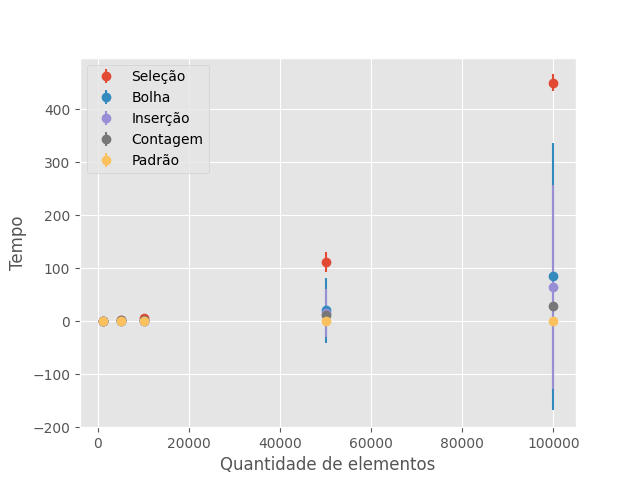
\includegraphics[width=8cm]{sizes.png}
    \caption{Gráfico elucidando o comportamento de cada algoritmo em tópico. No eixo x, há a quantidade de elementos; no y, o tempo médio gasto, em segundos, por cada algoritmo}
    \end{figure}

    \subsection{Ordenação prévia}
    \begin{figure}[h]
        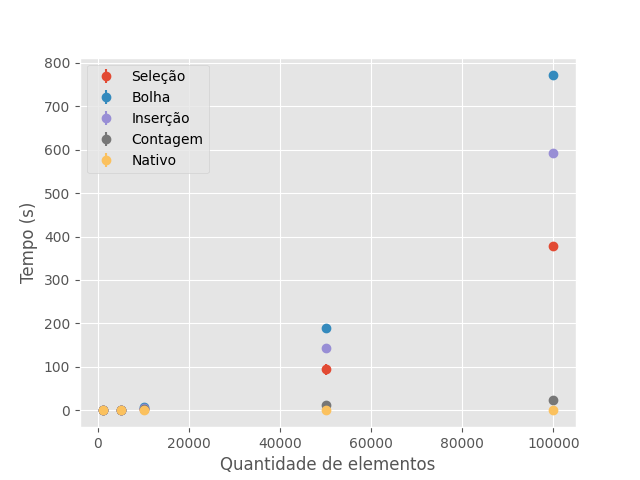
\includegraphics[width=8cm]{result_1717775798.8843806.png}
        \caption{Gráfico ilustrando o tempo médio 'gasto' dos algoritmos bolha e inserção em relação à taxa de ordenação inicial dos vetores.}
    \end{figure}

Como  previamente comentado, o algoritmo de bolha e o de inserção variam de acordo com a taxa de ordenação. Assim, em caso de ordenação inicial total, ambos os algoritmos adquirem um comportamento linear, uma vez que serão feitas $n$ comparações até que o algoritmo detecte que a lista já se encontra ordenada e, consequentemente, parará.
